\section{Alloy Modeling} \label{sec:alloy}

\subsection{Alloy Code} \label{code}
\lstinputlisting[language=alloy]{Alloy/RASD_Alloy_2.als}

\clearpage

\subsection{Worlds generated} \label{world}

The following images will show you the world generated from the execution of the predicate showAll(), ShowLockedCar() and ShowUnlockedCar(), respectively.

\begin{figure}[htbp]
\centering
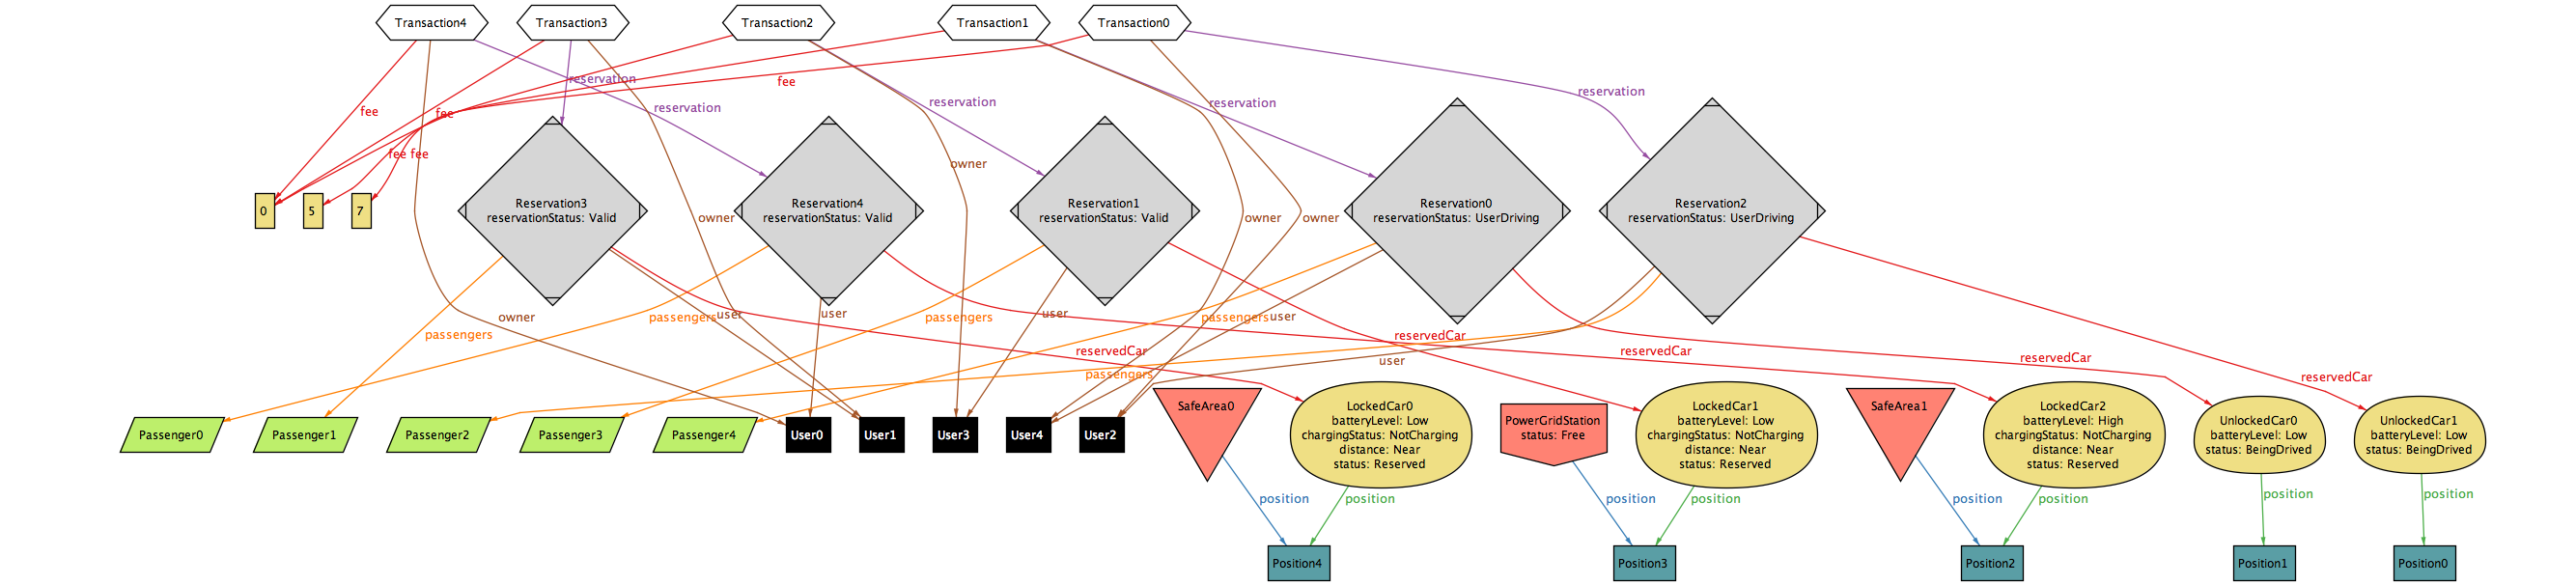
\includegraphics[width=1.5\textwidth, angle=90]{Alloy/showAll.png}
\caption{World generated from the execution of predicate showAll()}
\end{figure}
\clearpage

\begin{figure}[htbp]
\centering
\includegraphics[width=1.5\textwidth, angle=90]{Alloy/ShowLockedCar.png}
\caption{World generated from the execution of predicate ShowLockedCar()}
\end{figure}
\clearpage

\begin{figure}[htbp]
\centering
\includegraphics[width=1.5\textwidth, angle=90]{Alloy/ShowUnlockedCar}
\caption{World generated from the execution of predicate ShowUnlockedCar()}
\end{figure}
\clearpage